\documentclass[a4paper, 12pt]{article}

% Margins
% \usepackage[margin=2.5cm]{geometry}
\usepackage[top=1in,right=1.3in,left=1.3in,bottom=1in]{geometry}

% Headers and footers.
% useful options:
%   \thepage : the current page
%   \thispagestyle{empty} : kill header/footer on current page
\usepackage{fancyhdr}
% \lhead{Left Header}
% \chead{Center Header}
% \rhead{Right Header}
% \lfoot{Left Footer}
% \cfoot{Center Footer}
% \rfoot{Right Header}

% Control page header/footer.
% \pagestyle{plain} % No headers/footers.
% \pagestyle{headings} % Simple
\pagestyle{fancy}

% From Wim's. Don't know what they do
% \usepackage[T1]{fontenc}
% \usepackage{tgbonum}

% Simpler tables
\usepackage{tabularx}

% Muliple rows
\usepackage{multirow}

% Images
\usepackage{graphicx}

% Basic math stuff.
\usepackage{mathtools}
\usepackage{amsmath}

% Allows us to use .eps files.
% pdflatex --shell-escape --synctex=1 file.tex
\usepackage{epstopdf}

% Images in figures.
\usepackage{subfig}

% Turns off page numbering.
%\pagestyle{empty}

% Make captions look better.
\usepackage{caption}
\captionsetup{margin=30pt,font=small,labelfont=bf}

% Colours
\usepackage[usenames,dvipsnames]{color}
\definecolor{MyLightGray}{gray}{.90}

% Font stuff
\usepackage{palatino} % A nice alternative to Computer Modern

\usepackage{parskip}
% \setlength{\parskip}{0.1in}
% \setlength{\parindent}{0in}

% Hyperlinks
\usepackage{hyperref}

% Code listings
\usepackage{listings}
\lstset{
	frame=single,
        basicstyle=\small\ttfamily,
	keywordstyle=\color{black}\bfseries,
	commentstyle=\color{OliveGreen},
}

% To turn off section numbering:
% \section*{My Attempt}
%

% Tightly spaced lists, example:
% \begin{compactitem}
% \item ...
% \end{compactitem}
\usepackage{paralist}

% TODO
%\clearpage
%\newpage
%\linebreak

\begin{document}
\title{Particle Filters For Signal Processing}
\author{Benjamin Washington-Yule, Henry Jenkins}

% One or tather.
\maketitle
% \begin{titlepage}
\centering
\vspace*{\baselineskip}

\flushright\today\\
\centering
\rule{\textwidth}{1.6pt}\vspace*{-\baselineskip}\vspace*{2pt}
\rule{\textwidth}{0.4pt}\\[\baselineskip]

{\Huge \scshape

  Recursive Bayesian Estimation\\
  Techniques with\\
  Emphasis on the Particle Filter method.

}

\rule{\textwidth}{0.4pt}\vspace*{-\baselineskip}\vspace*{3.2pt}
\rule{\textwidth}{1.6pt}\\[\baselineskip]
{\scshape \large

  A Comparison Of\\
  Implementations\\

}


\vspace*{3\baselineskip}
{\Large

  {\scshape Benjamin Washington-Yule} (\emph{92646188})\\
  \url{byu17@uclive.ac.nz}\\
  \medskip\medskip
    {\scshape Henry Jenkins} (\emph{83238549})\\
    \url{hvj10@uclive.ac.nz}\\
}

\end{titlepage}


%\begin{abstract}
%The best abstract in the world.
%\end{abstract}


\begin{abstract}
This report describes the general Bayes filter and discusses two implementations
thereof: the Kalman filter and the particle filter. The framework for the Bayes filter is discussed
in detail, including the formulation of a state space model for a system. Two
application examples are chosen and simulated: image tracking and noise filtering.

The results for each are in line with expectations: the filter performance depends
on the accuracy of the model and the amount of measurement noise. Only the Kalman
filter implementation is functional, and it is not known why the particle filter
routine does not work. The implementation of the particle filter is examined
and compared to the Kalman implementation from a theoretical viewpoint. 

The results of the second example show that the Bayes filter can handle systems
where the noise is very high. It concludes with a short discussion where it is
concluded that the Kalman filter is sufficient for the majority of situations.
\end{abstract}

\section{Introduction}
The use of particle filters in signal processing is a comparatively new area of
research. The particle filter is a type of \emph{recursive Bayesian estimator},
also known as a \emph{Bayes filter}, and is closely related to another type
of Bayes filter called the \emph{Kalman filter}. Bayes filters find
applications in a wide range of areas, which includes among others,
\begin{compactitem}
\item Robotics, to infer position and orientation.
\item Computer vision, to track objects.
\item Medical fields, to extract information from noisy data.
\end{compactitem}
A Bayes filter is used in sensor and data fusion. It allows sensor measurements
to be combined with a state model to accurately track the state of a system.

The particle filter differs from the Kalman in the assumptions that are made
about the underlying system model and sensor noise. A more rigorous discussion
of these differences is found in Section \ref{sec:background} but the particle filter
can be generally described as having looser requirements, i.e., fewer
assumptions must be made about the model and sensor noise for a particle filter.
This may mean that in some cases a particle filter will succeed where a Kalman fails.
\section{Background}

\subsection{Bayes Filter}
Both particle and Kalman filters are types of Bayes filters. A Bayes filter,
or \emph{recursive Bayesian estimator}, provides a probabilistic framework
for estimation, but cannot be instantiated itself. To use terminology correctly:
particle and Kalman filters are implementations of the generic Bayes filter. As
such, they share very similar properties.

\subsubsection{State Space}
A Bayes filter is used for estimating the \emph{state} of a dynamic system from
noisey sensor measurements. The dynamic system is described by the state
vector $\textbf{x}$, and the following generic notation is used.

\begin{math}
\mathbf{x}_{t}\quad\quad\quad\textrm{state at time t} \\
\mathbf{z}_{t}\quad\quad\quad\textrm{observation at time t} \\
\mathbf{u}_{t}\quad\quad\quad\textrm{system input at time t}
\end{math}

Note that all of the state variables are vectors, indicating that a system can
have multiple states, observations and inputs. To illustrate how a system can be
decomposed into its state space consider the spring-mass-damper system shown in
Figure \ref{fig:spring-mass-damper}. The state of the system is composed of two
variables: position $x$ and velocity $\dot{x}$. We can use Newton's second law
to develop a force balance equation:

\begin{math}
\sum{F} = ma \\\\
F_{spring} = -kp \\
F_{damper} = -C\dot{p} \\\\
\sum{F} = ma = m\ddot{p} = -C\dot{p} -kx \\\\
\implies m\ddot{p} + C\dot{p} + kx = u
\end{math}

And form the state vector thus:

\begin{equation}
    \mathbf{x} =
    \begin{bmatrix}
        p \\
        \dot{p}
    \end{bmatrix}
    =
    \begin{bmatrix}
        x_{1} \\
        x_{2}
    \end{bmatrix}
\end{equation}

From which we can create the state space,

\begin{align*}
    \mathbf{\dot{x}}
    &=
    \begin{bmatrix}
        \dot{p} \\
        \ddot{p}
    \end{bmatrix} \\
    &=
    \begin{bmatrix}
        \dot{x} \\
        \frac{C}{M}\dot{p} - \frac{k}{M}p
    \end{bmatrix} \\
    &=
    \begin{bmatrix}
        x_{1} \\
        \frac{C}{M}x_{2} - \frac{k}{M}x_{1} - u
    \end{bmatrix} \\
    &=
    \begin{bmatrix}
        0 & 1\\
        \frac{-k}{M} & \frac{-C}{M} \\
    \end{bmatrix}
    \begin{bmatrix}
        x_{1} \\
        x_{2}
    \end{bmatrix}
    +
    \begin{bmatrix}
        0 \\
        1
    \end{bmatrix}
    u
\end{align*}
Which implies an overall state space,
\begin{equation}
\mathbf{\dot{x}} = \mathbf{A}\mathbf{x} + \mathbf{B}u
\end{equation}

where

\begin{math}
    \mathbf{A} =
    \begin{bmatrix}
        0 & 1\\
        \frac{-k}{M} & \frac{-C}{M} \\
    \end{bmatrix}\textrm{,}\quad
    \mathbf{B} =
    \begin{bmatrix}
        0 \\
        1
    \end{bmatrix}
\end{math}

We model the sensors similarly. The values of the matrices depend on which modes
we are able to observe. In this example we have said that we can observe position,
but not velocity. Our sensor vector is therefore simply a scalar value equal to
the first mode (position) of the system:

\begin{equation}
    \mathbf{z} =
    \begin{bmatrix}
        z
    \end{bmatrix}
    = x_{1}
\end{equation}

and the state space equations are therefore:

\begin{equation}
    z =
    \begin{bmatrix}
        1 & 0
    \end{bmatrix}
    \begin{bmatrix}
        x_{1} \\
        x_{2}
    \end{bmatrix}
    +
    \begin{bmatrix}
        0 \\
        0
    \end{bmatrix}
    u
\end{equation}

which we write using the usual state space notation.

\begin{equation}
z = \mathbf{C}\mathbf{x} + \mathbf{D}u
\end{equation}

Even though we have the system in state space form, it is not quite ready for
use as a model for a Bayes filter. There is a subtle change in the form of equations
\ref{eq:TODO} and \ref{eq:TODO} when used with a discrete system. The changes are shown here
without justification.\footnote{TODO}

\begin{equation}
\mathbf{x_{t+1}} = \mathbf{F}\mathbf{x_{t}} + \mathbf{G}u_{t}
\end{equation}

\begin{equation}
z_{t} = \mathbf{H}\mathbf{x_{t}} + \mathbf{J}u_{t}
\end{equation}

where

\begin{math}
    \mathbf{F} = \mathrm{\Delta t}\mathbf{A} + \mathbf{I_{4}}
    \textrm{,}\quad\\
    \mathbf{G} = \mathrm{\Delta t}\mathbf{B}
    \textrm{,}\quad\\
    \mathbf{H} = \mathbf{C}
    \textrm{,}\quad\\
    \mathbf{J} = \mathbf{D}
\end{math}

These are the key equations used in both the particle and Kalman filtering
algorithms.

Although the derivations of these state space forms are long-winded, the
formation of the state space is an important step for a Bayes filter.

\subsubsection{Estimation Process}
The aim of the Bayes filter is to find the belief about the current state.

\begin{math}
Bel(\mathbf{x}_{t}) = p(\mathbf{x}_{t} | \mathbf{z}_{1}, \mathbf{z}_{2}, \dots
, \mathbf{z}_{t})
\end{math}

that is, the probability of $\mathbf{x}_{t}$ given all the data we've seen so far.
Roughly speaking, the belief answers the question \emph{What is the probability
that the cart is at location x if the history of sensor measurements is
$\mathbf{z}_{1}, \mathbf{z}_{2}, \dots, \mathbf{z}_{t}$?} for all possible
locations.

The number of observations grows with time. To make the computation tractable,
Bayes filters assumet the dynamic system is \emph{Markov}\footnote{TODO:
explanation of a Markov process}, the result of this is that we assume that the
current state $\mathbf{x}_{t}$ contains all relevent information. Returning to
the example given previously, the Markov assumption implies that sensor measurements
depend only on an objects current physical location and that an object's location at
time $t$ depends only on the previous state $\mathbf{x}_{t-1}$. That is, states
before $\mathbf{x}_{t-1}$ provide no additional information under this assumption.

With this assumption, the belief function simplifies to that shown in
Equation \ref{eq:markov-belief}.

\begin{equation}\label{eq:markov-belief}
Bel(\mathbf{x}_{t}) = p(\mathbf{x}_{t} | \mathbf{z}_{t})
\end{equation}

\subsubsection{Updating the Bayes Filter}
Whenever a sensor provides a new observation $\mathbf{z}_{t}$\footnote{TODO:
remember that often z\_t is simpy a scalar}, the filter predicts state according
to \ref{eq:predict}. Note that the new sensor observation is not used in this step.

\begin{equation}\label{bayes-predict}
p(\mathbf{x}_{t} | \mathbf{z}_{t-1}) = \int{p(\mathbf{x}_{t} | \mathbf{x}_{t-1})
p(\mathbf{x}_{t} | \mathbf{z}_{t-1})\mathrm{d}\mathbf{x}_{t-1}}
\end{equation}

The filter then corrects the predicted estimate using the new sensor observation
according to \ref{eq:update}

\begin{align}\label{bayes-update}
    p(\mathbf{x}_{t} | \mathbf{z}_{t}) &=
    \frac
    {p(\mathbf{z}_{t} | \mathbf{x}_{t})p(\mathbf{x}_{t} | \mathbf{z}_{t-1})}
    {p(\mathbf{z}_{t} | \mathbf{z}_{t-1}}\\\\
    &=
    \alpha p(\mathbf{z}_{t} | \mathbf{x}_{t})p(\mathbf{x}_{t} | \mathbf{z}_{t-1})
\end{align}

%TODO make a comparison to Bayes Rule

It is often difficult to understand exactly what this all means just by looking at
Equations TODO through TODO, and a more qualitative description can clarify things.

$p(\mathbf{z}_{t} | \mathbf{x}_{t})$ is the perceptual model. It is the probability
of seeing a particular observation given that the system is in some state
$\mathbf{x}_{t}$ at time $t$. Using the previous example, it describes the
likelihood of making observation $z$ given that the cart is at location $x$.
The distribution is a property of a given sensor.

% TODO if filling required: to plots of good vs bad sensors.

$p(\mathbf{x}_{t} | \mathbf{x}_{t-1})$ is sometimes referred to as the action
model and describes the system dynamics. This is why it is essential to formulate
a state space model of the system under examination, as this is what is used to
formulate the distribution.

At this point it is worth iterating that Bayes filters only provide a
probabilistic framework for recursive state estimation and that implementing
a Bayes filter required specifying both perceptual model
$p(\mathbf{z}_{t} | \mathbf{x}_{t})$, the system dynamics
$p(\mathbf{x}_{t} | \mathbf{x}_{t+1})$ and the representation of the Belief
$p(\mathbf{x}_{t} | \mathbf{z}_{t})$.

\subsection{The Kalman Implementation}
The Kalman filter implementation utilises the specified state space system
model described in Section \ref{sec:TODO}. It is assumed that process noise
is added to the state update model thus:

\begin{equation}
\mathbf{x}_{t+1} = \mathbf{Fx}_{t} \mathbf{Bu}_{t} + \mathbf{w}_t
\end{equation}

Where $\mathbf{w}_t$ is zero mean, normally-distributed noise with convariance
$\mathbf{Q}$, i.e., $\mathbf{w}_{t} \sim N(0, \mathbf{Q})$.

Measurements are made by observing system state thus,

\begin{equation}
\mathbf{z}_{t} = \mathbf{Hx}_{t} + \mathbf{v}_t
\end{equation}

where $\mathbf{v}_{t} \sim N(0, \mathbf{R})$ and $\mathbf{R}$ is the
noise convariance.

\subsubsection{Prediciton}
The next state is predicted blindly according to supplied state model,

\begin{equation}
\mathbf{x}_{t|t-1} = \mathbf{Fx}_{t-1|t-1} + \mathbf{Bu}_{t}
\end{equation}

and the estimate covariance updated according to,

\begin{equation}
\mathbf{P}_{t|t-1} = \mathbf{FP_{t-1|t-1}F^{T}} + \mathbf{Q}
\end{equation}

\subsubsection{Updating}

\begin{math}
\tilde{\textbf{y}}_k = \textbf{z}_k - \textbf{H}_k\hat{\textbf{x}}_{k|k-1}\\
\textbf{S}_k = \textbf{H}_k \textbf{P}_{k|k-1} \textbf{H}_k^\text{T} + \textbf{R}_k\\
\textbf{K}_k = \textbf{P}_{k|k-1}\textbf{H}_k^\text{T}\textbf{S}_k^{-1}\\
\hat{\textbf{x}}_{k|k} = \hat{\textbf{x}}_{k|k-1} + \textbf{K}_k\tilde{\textbf{y}}_k\\
\textbf{P}_{k|k} = (I - \textbf{K}_k \textbf{H}_k) \textbf{P}_{k|k-1}
\end{math}

\subsection{The Particle Filter Implementation}

% TODO particle filtering algorithm
    

\section{Application: Image Tracking}
Image tracking is a common common application for Bayes filters. A certain aspect or
object in an image is to be tracked, and the goal is to use a state
model and sensor measurements to estimate its state. In the case of image
tracking the observations are usually generated by some sort of image processing
operation that identifies objects in an image. The noise inherent in these measurements
comes from the imperfect nature of this processing.

Two example video sequences were chosen to implement object tracking. Both consist
of a single object (a ball) falling past a uniform background and hitting the ground
and bouncing a certain number of times. Video sequences of this form are the easiest
to track because
\begin{compactitem}
\item The object (ball) is visible for the entire duration.
\item There is only a single moving object.
\item There are a number of frames at the start of the sequence in which the
ball is not visible.
\end{compactitem}
The last point is important as it allows an accurate representation of the background
to be stored by averaging the first $n$ frames in which the object is not present.
The measurements are then obtained by subtracting the background from this image.

\subsection{Observations}
The Bayes filter estimates state using (noisy) sensor measurements. In our case
the ``sensor" is an image processing routine that attempts to identify the ball.
No feedback is used in this operation so the sensor may end up simply identifying
the largest, or most circular objects in some cases. Detection errors like these
are what represent the measurement noise.

The observation algorithm used to detect the ball in each frame is shown in
pseudo-code in Listing \ref{lst:obs}.

\begin{lstlisting}[language=Matlab, label=lst:obs,
caption=Implementation of observation routine.]
% Subtract background from frame
frame = frame - background;

% Background pixels = 0, Object pixels = 1
for pixel in frame:
    if pixel != 0 then pixel = 1;

% Clean up the shape of all objects.
frame = erode(frame);

our_object = largest_object(frame)

if object is None then exit

return object
\end{lstlisting}

The measurement routine is in essence a background-subtraction followed by some
inbuilt Matlab functions for identifying similar regions.\footnote{TODO quick
explanation of the functions bwmorph, bwlabel, regionprops}. The result of a
typical measurement is shown in Figure \ref{fig:observation}.

\begin{figure}[h]
\centering
\subfloat[A]{
    \label{fig:untouched}
    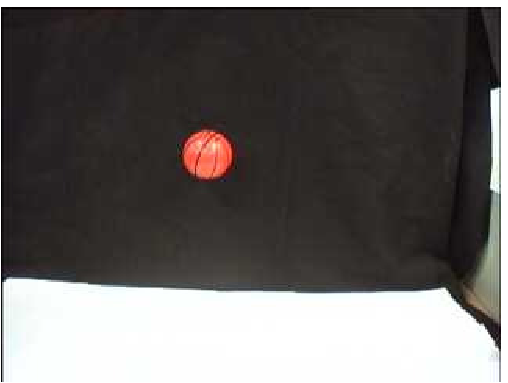
\includegraphics[width=0.4\textwidth]{images/observation/untouched}
}
\subfloat[B]{
    \label{fig:subtracted}
    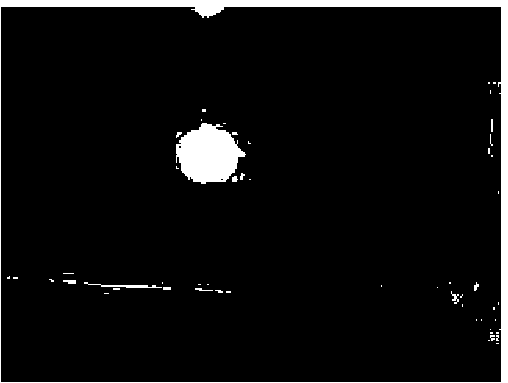
\includegraphics[width=0.4\textwidth]{images/observation/subtracted}
} \\
\subfloat[C]{
    \label{fig:marked}
    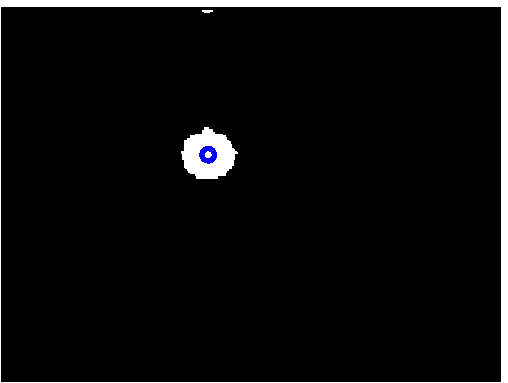
\includegraphics[width=0.4\textwidth]{images/observation/marked}
}
\subfloat[D]{
    \label{fig:identified}
    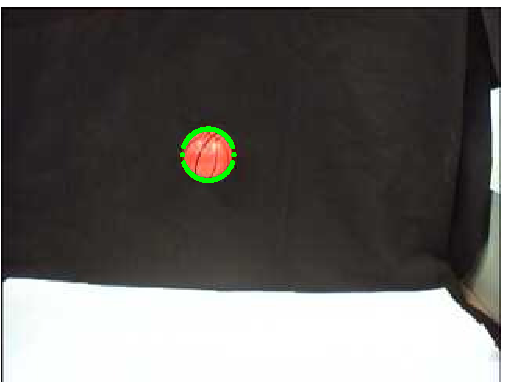
\includegraphics[width=0.4\textwidth]{images/observation/identified}
}
\caption{A standalone pineapple scaled to half the text-width.}
\label{fig:observation}
\end{figure}

Figure \ref{fig:untouched} shows the original frame. The ball's motion is in
a downward direction. Since we have already found the background for all frames,
we can perform a subtraction to obtain the modified frame shown in Figure
\ref{fig:subtracted}. It is then cleaned up using inbuilt Matlab image processing
functions, and this same family of functions is also used to identify the contiguous
pixels which form the ball. As a result of the eroded image's maintaining
a circular geometry, we simply measure the ball's centre as the centre of the
white area. Were the frame to be noisier, we may lose the circular outline and
the measured centre may drift to a more incorrect value.

For illustration, the outline of the ball as measured is shown in Figure
\ref{fig:identified}. What appears to be a continuous green line is in fact
a series of green points equidistant from the measured centre using a radial
value returned from Matlab. Note again that even though the outline appears
very accurate in the chosen frame, it is possible for it to be slightly, or
completely off from the ball depending on the noise present in the image.

It is worth pointing out at this stage that such an accurate sensor eliminates
the need for a Bayes filter, as one can simply track the very accurate sensor
measurements. However, with only a small amount of additional noise, or the ball's
being obstructed for several frames, we would quickly necessitate a Bayes filter.
To be able to implement and test Bayesian estimation, an additional ability was
built into the measurement function to intentionally inject noise. 

The entire measurement routine was implemented as a Matlab function which
returned the coordinates (pixel locations) of the measured centre of the ball
in a given frame. This value is then used by the state space model of the system.

\subsection{State Space Model}
State space models, while important, are often extremely difficult to formulate
for real systems. However, because of the accurate sensor measurements we can
get away with an overly simplistic model, at least initially. The state space
that was chosen is shown in Equation \ref{eq:basket-state-space}. It consists
of the 2D position of the centre of the ball and the velocity in each direction.

\begin{equation}\label{eq:basket-state-space}
\mathbf{x} =
\begin{bmatrix}
x \\ y \\ \dot{x} \\ \dot{y}
\end{bmatrix}
\end{equation}

Where $x$ and $y$ are the x- and y-coordinates respectively, and the velocity
in each direction is represented by their derivatives $\dot{x}$ and $\dot{y}$.
The positional units are with respect the the size of the image, and the velocities
in pixels per second. Having higher-order aspects of the system such acceleration
in the state space serve little purpose in this example.

\subsubsection{State Update Equation}
The simplest non-trivial model that can be applied to this system is to model
the affect of gravity. Having a dynamical model which \emph{only} takes gravity
into account will of course, break down very quickly and is not realistic. However,
it serves as a simple test.

At each time step, the positions are updated as shown in Equations
\ref{eq:pos-update} and \ref{eq:pos-update},

\begin{align}
x_{t+1} = x_{t} + \dot{x}_{t} \\
y_{t+1} = y_{t} + \dot{y}_{t}
\end{align}

That is, at each time step the positions change by the current velocities.
The velocities are themselves updated according to,
\footnote{The astute reader may notice a
perceived discrepancy in the units
at this point. It was stated that velocities are in pixels/sec, but the time
steps occur much faster than this. This is precisely the reason for the
modifications to the state matrices in Section \ref{TODO}.
}

\ref{eq:pos-update} and \ref{eq:pos-update}.
\begin{align}
\dot{x}_{t+1} = 0 \\
\dot{y}_{t+1} = \dot{y}_{t} + g
\end{align}

That is, the velocity in the y-direction is incremented by the value of gravity
we choose and the velocity in the x direction remains unchanged.
It is important to keep in mind that this is simply a model we are building to
represent the behaviour of the
system; even though there is almost certainly some sideways movement of the ball,
it is probably suffice to model it as zero.

Using these equations we can begin to generate the state-space model for this
example.

\begin{align}
\mathbf{x_{t+1}} &=
\begin{bmatrix}
x_{t+1} \\ y_{t+1} \\ \dot{x}_{t+1} \\ \dot{y}_{t+1}
\end{bmatrix}
\\
&=
\begin{bmatrix}
x_{t} + \dot{x}_{t} \\ y_{t} + \dot{y}_{t} \\ 0 \\ g
\end{bmatrix}
\\
&=
\begin{bmatrix}
1 & 0 & 1 & 0 \\ 0 & 1 & 0 & 1 \\ 0 & 0 & 1 & 0 \\ 0 & 0 & 0 & 1
\end{bmatrix}
\mathbf{x}_{t} + 
\begin{bmatrix}
0 \\ 0 \\ 0 \\ 1
\end{bmatrix}
g
\\
&=
\mathbf{Ax}_{t} + \mathbf{Bu}_{t}
\end{align}

Where (21) is the usual state-space form.

\subsection{Filtering Steps and Noise}
The Kalman filter implementation of the Bayes filter was used for testing, under
the conditions of the example, that is, a linear model and linear noise,
the Kalman and particle filter methods are expected to perform identically. As
stated in Section \ref{sec:TODO}, the Bayes filter has two distinct steps:
the prediction and update steps. The implementation of the two steps differs
for the Kalman and particle filter implementations, but are described generally
below.

In the prediction step we use our simple state
model to predict the state of the system in the next time step. Since we are using
such a simplistic model where the ball acts under a form of gravity, the predict
step is easy to picture. It simply says that the ball will have moved downward by
$g$ pixels at each time step. This model performs well when the ball does in fact
have a downward velocity, but as expected, breaks down when the ball hits the floor
or has an upward velocity.

The update step is where we use the latest sensor measurement to correct our
prediction. It incorporates the predicted state model and the observation. Naturally,
if these values were identical then there is no change in the update step.

In both of the two steps the noise was assumed to be Gaussian. During testing,
we simulated this noise by adding randomly distributed random numbers to both
the sensor measurements and the state update equations.

\subsection{Results}
The results for this example were not groundbreaking. The Kalman filter
implementation was first tested. As expected, the filter
tracked the object very closely while the ball had a downward trajectory, and
even when it did not, the filter still managed to stay very close. We can explain
this in terms of the (lack of) measurement noise; even when the state model broke down,
(i.e., when the ball hit the ground), the measurements were so accurate
that close tracking was still achieved.

\subsubsection{Simulated Noise}
To try and create a more realistic situation, we intentionally injected noise into
the sensor measurements and process updates. Adding additional noise to the measurement
step did not affect the tracking ability to a large extent. On the other hand,
adding only a small amount of noise to the state update step caused tracking to
become much worse. This is again entirely expected and came be easily explained
by considering our simple model. Adding noise to the update model causes two
detrimental effects, (a) the x position now changes due to noise and (b) the
effect of ``falling" under pixel gravity may now be exaggerated if a high or low
noise value is added to the model while the ball is in free-fall or rebound respectively.

Even with the added noise and the inaccurate model, close tracking was still
maintained. This can be put down to the simplicity of the actual system under
examination. A ball bouncing under gravity has only a single degree of freedom
and although the model is incorrect for half of duration of the video (while
the ball is rebounding), the measurements are still so clear that we can track
the ball accurately.

In order to prove that we simply were not following the measurements and
disregarding the state update, a final test was constructed where the measurement
noise was given an extremely high value ($\sigma = 10$) and the process noise set
to zero. When the simulation was run, tracking was started and maintained as
soon as the ball entered the frame and was moving downward, but was lost entirely
when the ball hit the ground. This is an encouraging result and shows two things:
\begin{compactitem}
\item Recursive Bayesian estimate relies on both the state model and the observations
\item If one of: the measurement noise is high or the model inaccurate, then the
other must be even more accurate to make up.
\end{compactitem}

% TODO qualatative table if filler needed

\subsubsection{Obstructions}
A second test of the filtering algorithm is to add an obstruction to the image.
This means that the object (ball) that we are trying to track ``disappears" from
for one or more frames then comes back into view. Unfortunately, the videos
had already been taken by this stage and time did not permit a reshoot with
an obstruction added. We were able to simulate this however, by simply dropping
measurements for one or more frames.

Implementing this simulated obstruction was simple, and required a change of
only a few lines of code. As a consequence of our overly simplistic model, the
tracking was only expected to work moving past the ``obstruction" in the
downward direction. This is indeed what was observed but it was interesting to
note just how well tracking was maintained moving past the ``obstruction" in
the downward direction. As soon as the ball disappeared, i.e., no measurement was
available, the state model of the system took over and tracked the ball down
though the obstruction. This highlights the strength of the Bayes filter, but also
the importance of an accurate model.

\subsection{Particle Filter Implementation}
Unfortunately the algorithm developed for the particle filter method did not work.
It is still not known why but we can make some assumptions about what would
have happened:
\begin{compactitem}
\item The measurements would have been identical as this was independent of the
filter implementation.
\item The tracking would have been as good or better then the Kalman implementation
due to the particle filter's ability to deal with both Gaussian and non-Gaussian
noise.
\end{compactitem}

\section{Application: Filtering}
We developed a second example in order to further test the properties of Bayes
filters. The image tracking example, while realistic, did not allow control of
the system, as it was simply a collection of frames that could not be changed.
Our second example involved developing a system that we completely specify, i.e.,
we have exact knowledge of its dynamical model because we created it.

The system used in the example is the spring-mass-damper described in Section
\ref{sec:TODO}. The state space derivation is already given. We could now
analyse this system in a way we could not with the image tracking example. The
goal of this example can be stated thus: given a state-space model that is
very accurate (by definition it is perfectly accurate), and a random input
into this system, how much sensor noise can we tolerate before tracking is lost?

\subsection{Noise}
Measurement noise in the system is by definition zero, as we can observe the
state without error. To simulate noise in the measurements, a normally-distributed
random number was added to the measurement at each time step. Manually adding this
error also means that we have knowledge of the noise variance (as we specify it).

\subsection{Results}
The Bayes filter was implemented as a Kalman filter becuase of the difficulties
obtaining resilts using the particle filter implementaiton.

Figure \ref{fig:filter} shows the results of the Bayes filter with extremely
high measurement noise ($\sigma = 10$). The true state is shown in Figure
\ref{fig:true-state}. It is a damped system starting at position $p = 10$ with
an additional random input, which is unknown to the sensor. Figure \ref{fig:measured-state}
shows the measured state. Because of the amount of noise it is almost impossible
to make out the original signal\footnote{This is typical of signals obtained
from patients in which the blood-glucose level is to be tracked.}. Finally,
Figure \ref{fig:estimated-state} shows the output of the Bayes filter.

\begin{figure}[h]
\centering
\subfloat[A]{
    \label{fig:untouched}
    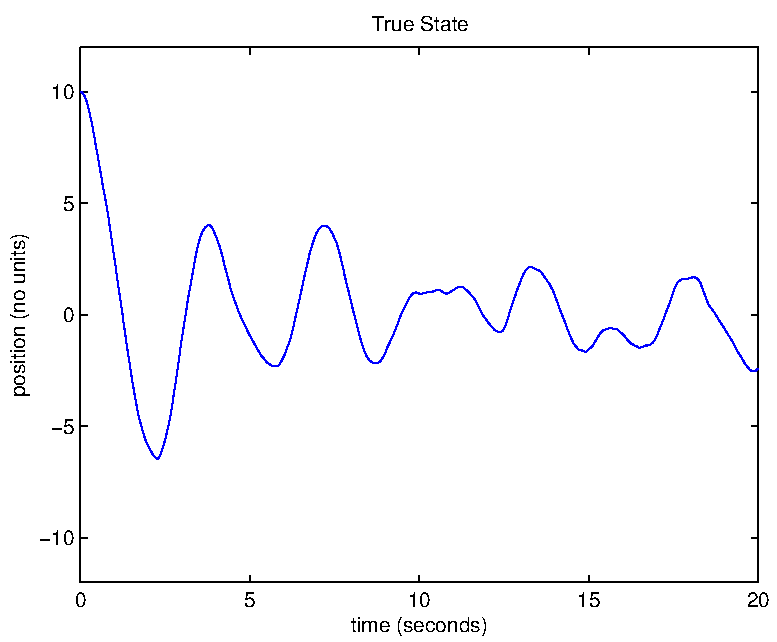
\includegraphics[width=0.6\textwidth]{images/true-state}
}
\subfloat[B]{
    \label{fig:subtracted}
    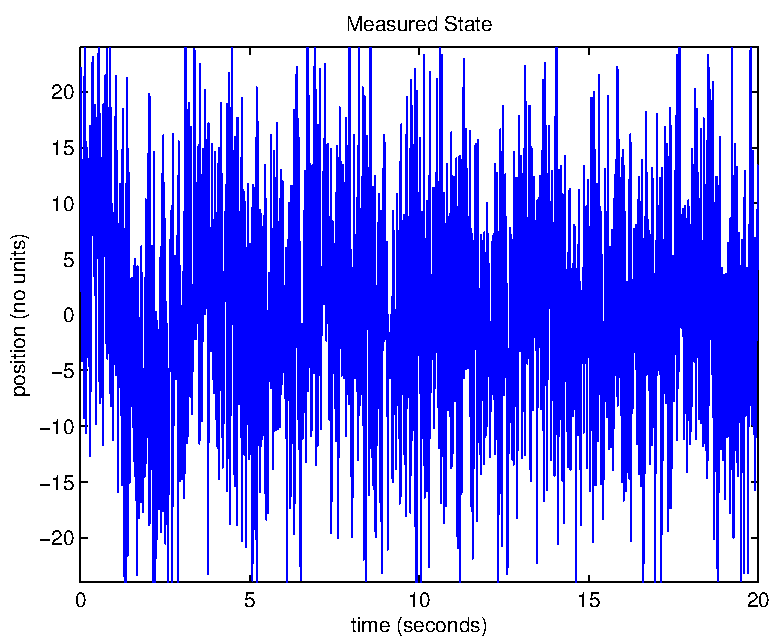
\includegraphics[width=0.6\textwidth]{images/measured-state}
}
\subfloat[C]{
    \label{fig:marked}
    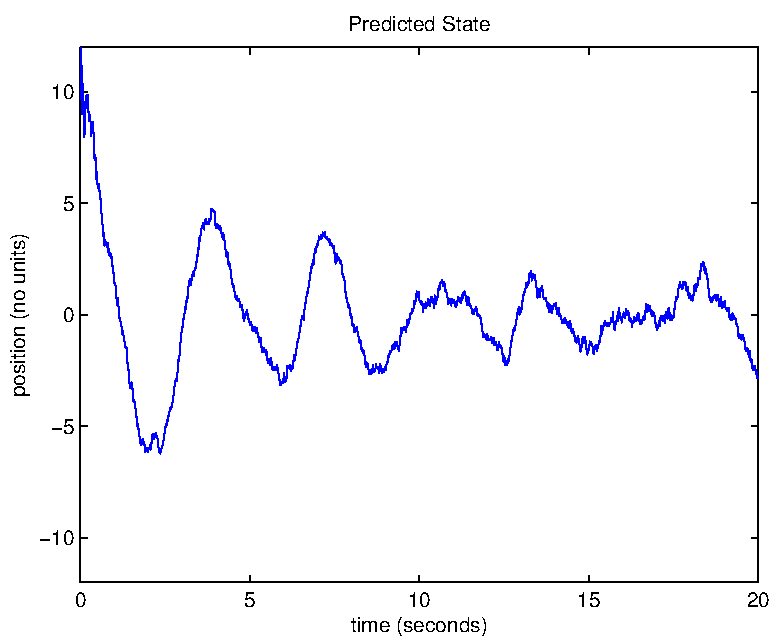
\includegraphics[width=0.6\textwidth]{images/estimated-state}
}
\caption{A standalone pineapple scaled to half the text-width.}
\label{fig:filter}
\end{figure}

The output maintains remarkably close tracking of the input, or stated in a
way more fitting for the example: the noise has been almost completely filtered
from the measured signal. As remarkable as this example be, it is contrived and
it is important to note the following:
\begin{compactitem}
\item Measurement noise is randomly distributed and we are aware of this fact.
\item We know the measurement noise variance \emph{exactly}.
\item We know the process noise variance \emph{exactly}.
\end{compactitem}
If either of these change, then tracking is expected to become less accurate, or
at worst, lost completely. To test this hypothesis, the true noise variance was
changed to ($\sigma = 5$) while our belief of the variance was in fact at
($\sigma = 2$). The result is shown in Figure \ref{fig:filter-bad}. It is
visually obvious that the state is not being tracked accurately, highlighting
the importance of characterising the sensors so that the noise variance is
known.

\begin{figure}[h]
\centering
\subfloat[A]{
    \label{fig:untouched}
    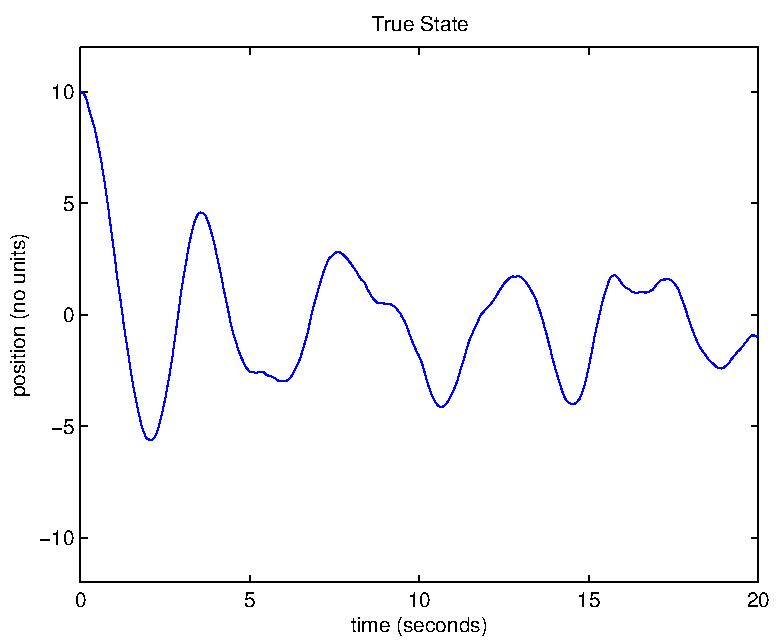
\includegraphics[width=0.5\textwidth]{images/true-state-bad}
}
\subfloat[B]{
    \label{fig:subtracted}
    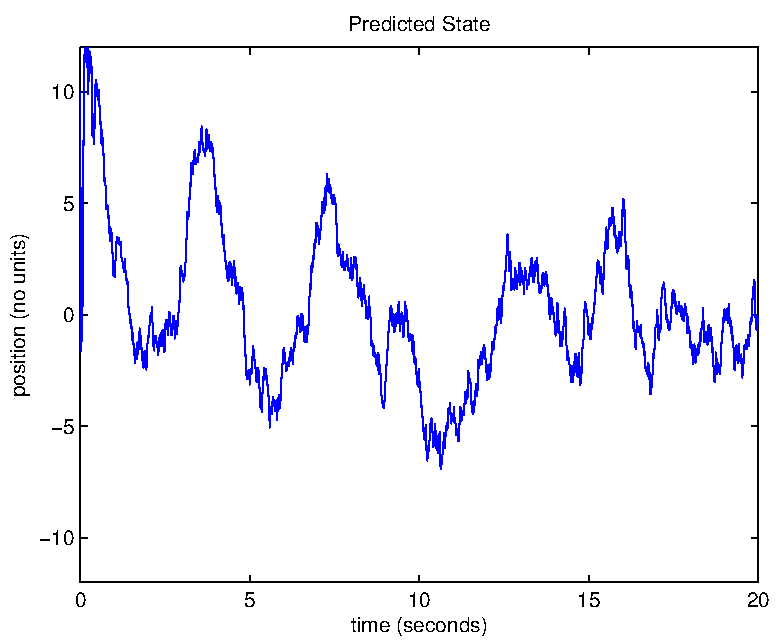
\includegraphics[width=0.5\textwidth]{images/estimated-state-bad}
}
\caption{A standalone pineapple scaled to half the text-width.}
\label{fig:filter-bad}
\end{figure}

The relative error between the true and estimated states for different values
of noise variance error is shown in Figure \ref{fig:noise-error}. As expected,
the more incorrect we are about the sensor noise variance, the worse tracking
becomes.

\begin{figure}[h]
\centering
\subfloat[A]{
    \label{fig:untouched}
    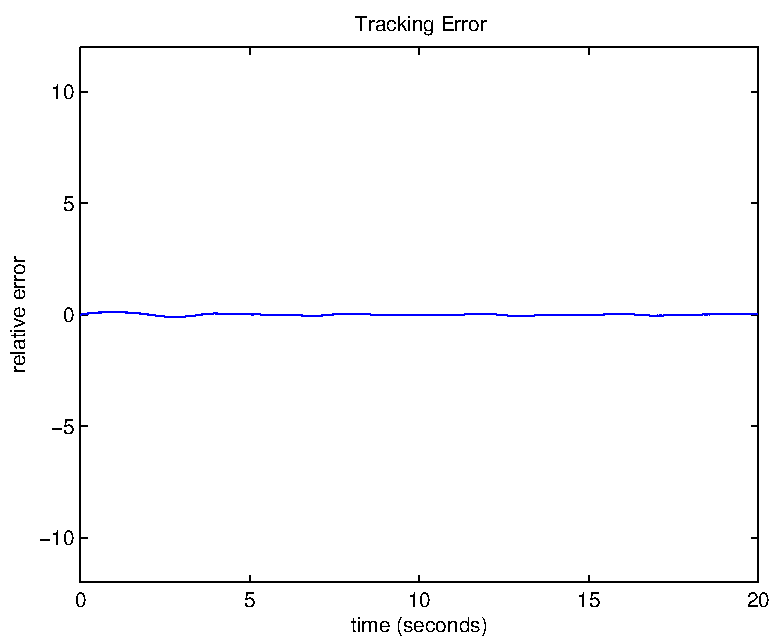
\includegraphics[width=0.3\textwidth]{images/error-state-0}
}
\subfloat[B]{
    \label{fig:subtracted}
    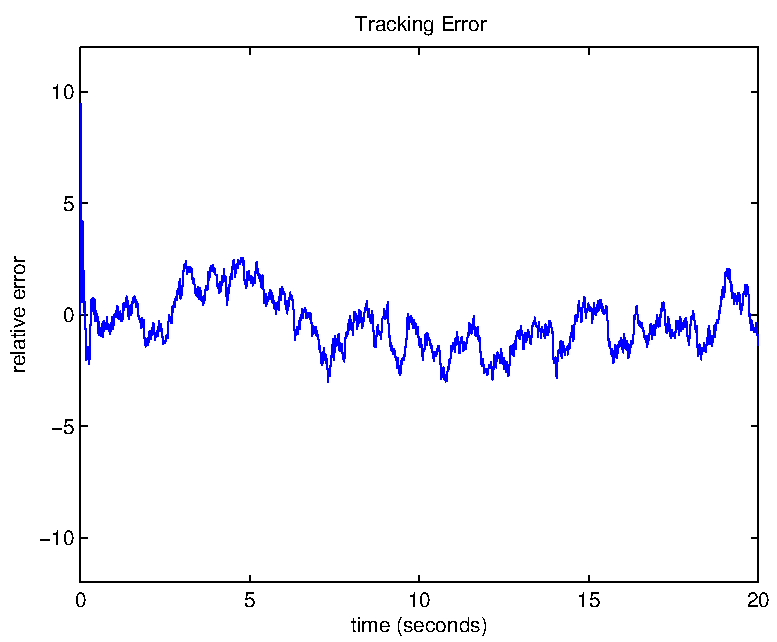
\includegraphics[width=0.3\textwidth]{images/error-state-10}
}
\subfloat[C]{
    \label{fig:marked}
    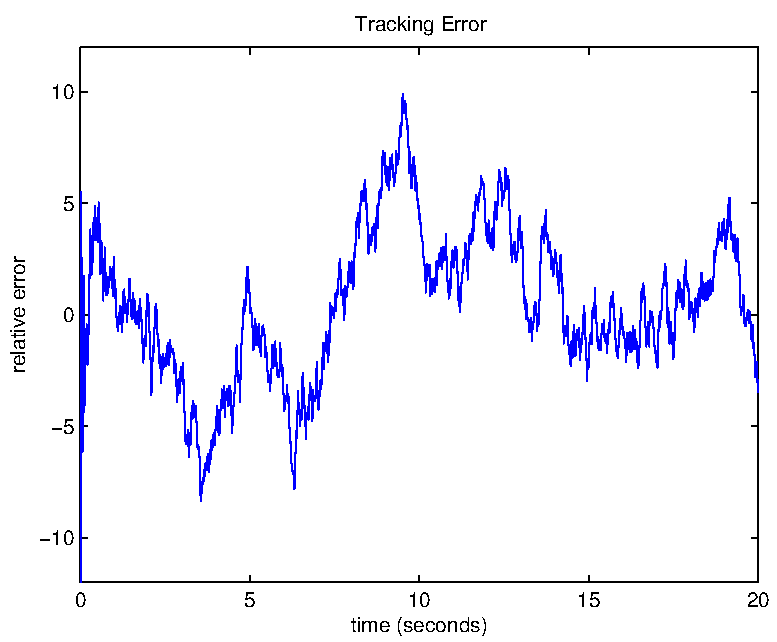
\includegraphics[width=0.3\textwidth]{images/error-state-20}
}
\caption{A standalone pineapple scaled to half the text-width.}
\label{fig:filter}
\end{figure}

\subsubsection{Particle Filter Implementation}
Even though the particle filter implementation did not work, we attempted to
create a non-linear state model, expecting the Kalman filter to fail because
of its inability to handle non-linearity in the system model.

The state model was changed to a simple non-linear system modelling a pendulum.
The derivation is omitted and only the final state-space equations are shown.

\begin{equation}
\mathbf{x}(t+1) =
\begin{pmatrix}
x_{1}(t+1) \\ x_{2}(t+1)
\end{pmatrix}
=
\mathbf{f}(t, \mathbf{x}(t)) =
\begin{pmatrix}
x_{2}(t) \\ \alpha \sin x_{1}(t) - \beta x_{2}(t)
\end{pmatrix}
\end{equation}

The same procedure was used for this new non-linear system. Unexpectedly however,
the Kalman implementation of the Bayes filter continued to work correctly.
It is unknown why this happened, but one assumption to be made is that if the
Kalman implementation functioned correctly, then the particle filter implementation
would certainly function too.


\section{Conclusions}

The results observed for both application examples are in line with what was
expected, with the exception of the Kalman filter implementation's not failing
when presented with a non-linear system model.

The image tracking application was successful despite the overly simplistic 
model used. However, it is important not to draw unwarranted conclusions 
from this example and assume that an
inaccurate system model will not affect the Bayes filter's ability to track an
image. On the contrary, the results show that an inaccurate model is
more detrimental than high measurement noise. If the first application example 
was even slightly
more complex, e.g., giving the ball a second degree of freedom, then our
overly simplistic model that only takes gravity into account would certainly not
work as intended.

The second filtering application example showed that we are able to obtain very accurate tracking 
(filtering) even in the presence of atypically high sensor noise, but that this
is only because we can characterize the noise accurately. We conclude that 
recursive Bayesian estimation is an extremely powerful tool, but that its power
depends on
\begin{compactitem}
\item The accuracy of the sensor model.
\item The accuracy of the dynamical model.
\end{compactitem}
i.e., a Bayes filter is only as accurate as the model and the characterization 
of the noise.

If either of these are below a certain threshold (dependent on the situation) 
then the other must be very accurate to compensate or tracking will be lost
entirely.

\subsection{Particle Filter Implementation}
We conclude that the particle filter implementation of the Bayes filter is 
difficult to implement at best, especially in Matlab. We come to this conclusion
after observing the following:
\begin{compactitem}
\item There is very little reference material on the internet about particle filters
in software, the few that do exist are implemented in C.
\item Our Matlab implementation did not appear to work.
\item Many papers that mention particle filtering, in fact write the implementation
using an alternate (usually Kalman) implementation.
\end{compactitem}
It should be pointed out that we are unsure whether our particle filter implementation
was close to, or far from functioning. Given more time, it would be desirable to 
investigate this further.

Even without a working implementation, we have still built the framework for a
particle filter implementation. The system, dynamical and noise models are
all complete, and with further work, the particle filter predict and update
routines could easily be inserted into the code.

From all evidence we conclude that for all examples presented in this report, 
the particle filter implementation would produce results equal to or better than
our test Kalman implementation.

One point to note about the application described in Section \ref{sec:image-tracking}
is that if were we to employ a more accurate model for the balls motion, e.g., 
a model that takes into account the impulse from hitting the ground and a sudden change in velocity,
then it would likely become a very non-linear system which may eventually 
cause the Kalman implementation may break down, and a particle filter become necessary.
However, we have also observed that the Kalman filter can handle non-linearities so 
the particular threshold is unknown.

It appears that for most applications, the Kalman filter performs 
satisfactorily, even in the presence of slight non-linearity in the
system model. However, we assume that there exist models of sufficient complexity
that will benefit from the particle filter method.


% Bibliography. The "99" allows up to 99 entries apparently.
\begin{thebibliography}{99}
\bibitem{ref:example} Benjamin Washington-Yule, How to LaTex, 1999, Harper Collins
\end{thebibliography}

\end{document}
